\chapter{Basi teoriche}
\label{cap:teoria}
\intro{Per comprendere al meglio gli argomenti trattati nel capitolo successivo è necessaria un'introduzione teorica}

\section{Machine learning}
Il machine learning è un'applicazione della statistica che si concentra sullo sviluppo di algoritmi in grado di imparare dai dati che vengono loro forniti in input.
Da un punto di vista più filosofico il machine learning è interessante perché sviluppando la nostra conoscenza su di esso stiamo di conseguenza migliorando la nostra comprensione dei principi su cui si sorregge l'intelligenza \footcite[p.~97]{Goodfellow-et-al-2016}.
Gli algoritmi di machine learning si suddividono in due categorie principali:

\begin{itemize}
    \item apprendimento supervisionato
    \item apprendimento non supervisionato 
\end{itemize}

\subsection{apprendimento supervisionato}
Gli algoritmi che appartengono a questa categoria apprendono quali risultati generare seguendo la guida di un set di dati etichettati e con un output predefinito\footcite{site:machine-learning}.

\subsection{apprendimento non supervisionato}
Gli algoritmi non supervisionati, anche conosciuti come apprendimento automatico, analizzano e raggruppano dataset non etichettati. Questi algoritmi riconoscono raggruppamenti di dati (cluster) senza la necessità dell'intervento umano\footcite{site:machine-learning}.

\section{K-means}
Il K-means è un algoritmo non supervisionato che viene utilizzato per il clustering, ossia per la suddivisione del dataset in gruppi che contengono caratteristiche simili.
Suddivide un set di dati in gruppi simili sulla base della distanza tra i loro centroidi. 
Il centroide, è la media di tutti i punti presenti all'interno del cluster.

Il numero K sta a indicare quanti cluster dovranno essere assegnati dall'algoritmo, più il numero di cluster è elevato più essi saranno piccoli e dettagliati al contrario se i cluster sono pochi il risultato saranno dei cluster più grandi ma meno dettagliati.

Ad esempio se volessimo clusterizzare un insieme di animali composto da mammiferi e uccelli utilizzando K=2 l'algoritmo creerebbe due cluster uno contenente i mammiferi e uno gli uccelli (cluster grandi e poco dettagliati).
Se aumentassimo il numero di cluster l'algoritmo sarebbe in grado di essere più specifico andando a creare una quantità molto più elevata di cluster ben dettagliati contenenti meno elementi.
Quindi è importante scegliere con cura il numero iniziale K da assegnare, per semplificare questa operazione esistono dei metodi di supporto:
\begin{itemize}
    \item Il metodo del gomito sfrutta l’inerzia, ossia la somma delle distanze al quadrato dei punti dal centroide (SSE, Sum of Squared Errors). Con l'aumento dei cluster, l’inerzia diminuisce, ma dopo un certo punto, la riduzione diventa superflua, venendo a creare una curva a gomito. Il punto in cui la curva si piega indica il numero di cluster da utilizzare.
    
    \begin{figure}[!h] 
        \centering 
        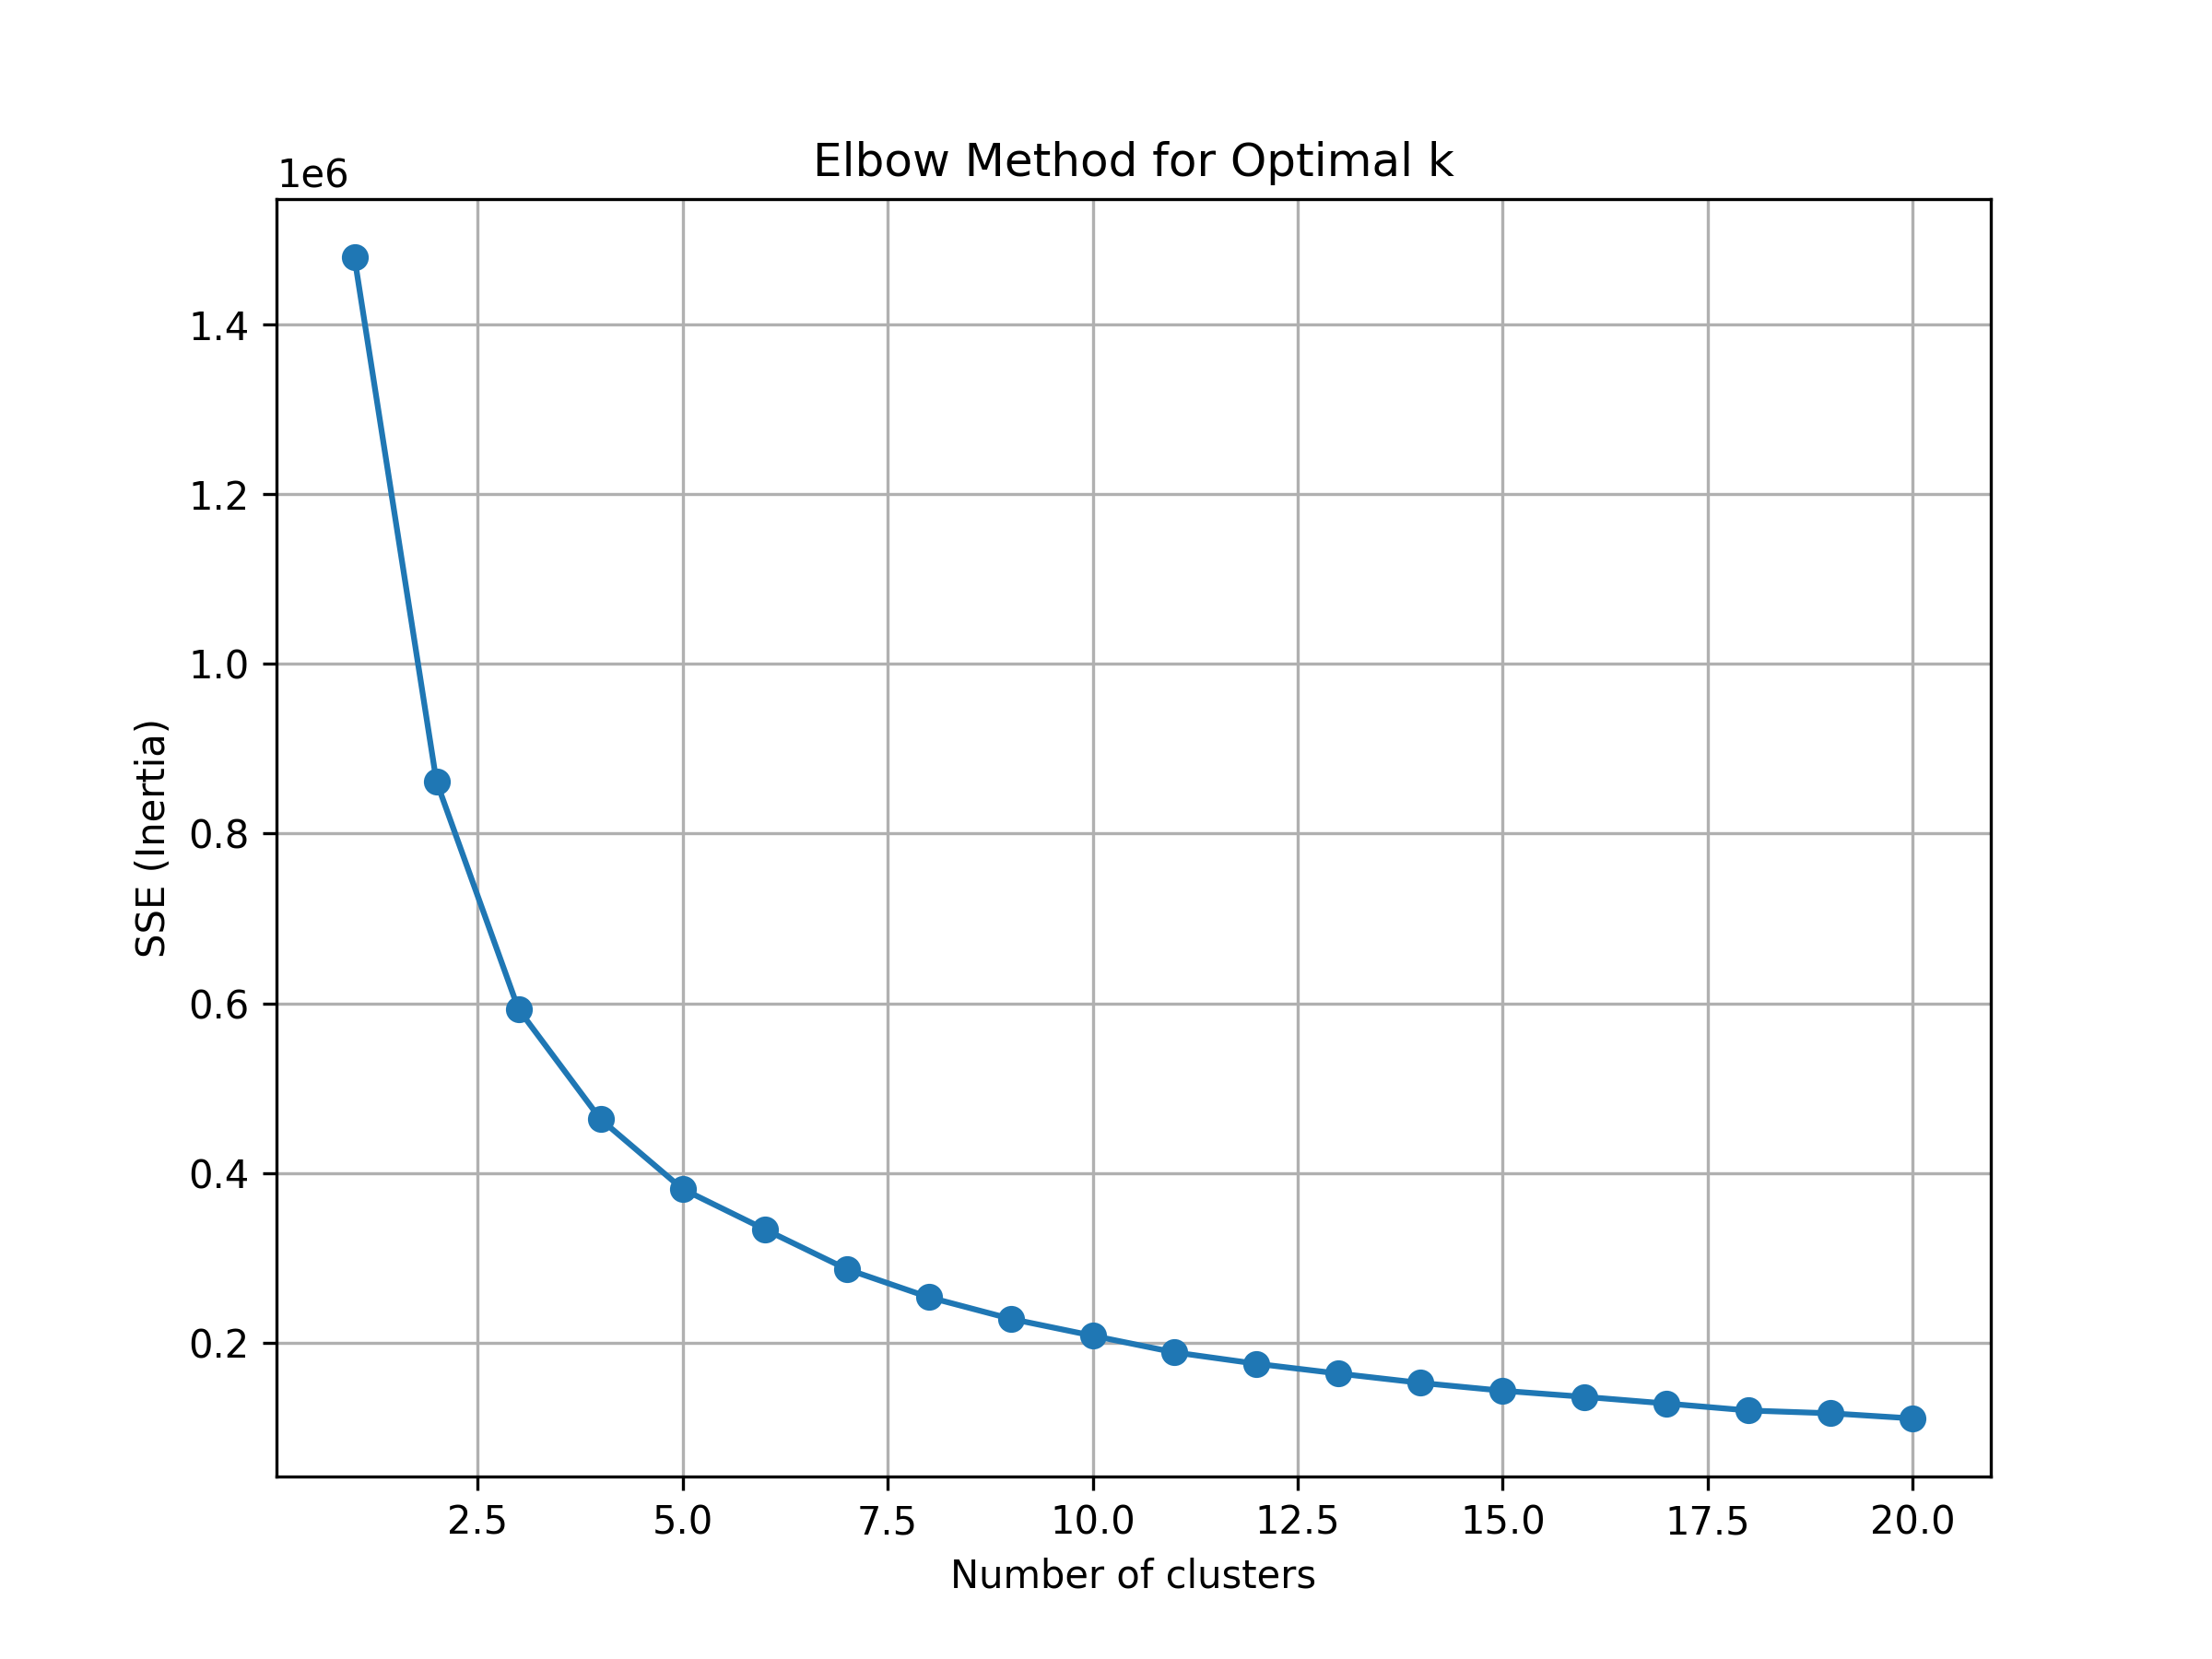
\includegraphics[width=0.7\columnwidth]{teoria/elbow_method.png} 
        \caption{Grafico rappresentante il metodo del gomito}
        \label{fig:gomito}
      \end{figure}

    \item Il Silhouette Score indica quanto i punti appartenenti a un cluster sono simili tra loro e quanto differiscono dai punti contenuti negli altri cluster.
    Varia tra -1 e 1, se il valore è vicino a 1 il punto è all'interno del suo cluster e ben separato dai cluster limitrofi, se è vicino a 0 il punto è confinante tra due cluster infine un valore negativo indica l'assegnazione a un cluster sbagliato.
\end{itemize}

%dovresti spiegare come funziona realmente ma vediamo che dice il prof

\section{PCA}
L'analisi dei componenti principali è un algoritmo non supervisionato in grado di estrarre le informazioni più rilevanti da dataset di grandi dimensioni, riducendo così la complessità del modello ed evitando che si presenti il fenomeno della "maledizione della dimensionalità"\footcite{site:PCA}.

\subsection{Maledizione della dimensionalità}
La maledizione della dimensionalità si verifica all'aumentare della dimensionalità dei dati: con l'aumentare delle dimensioni, il volume dello spazio aumenta in maniera esponenziale, rendendo difficile l'elaborazione da parte degli algoritmi di machine learning, che dovranno lavorare su dati molto sparsi con conseguenze negative per le prestazioni.

\section{feature}

\section{Deep learning}
Il deep learning è un processo di machine learning che sfrutta nodi interconnessi tra di loro (anche chiamati neuroni) in una struttura a strati ispirata al cervello umano (da qui neural network).
In genere consistono di un sistema adattivo utilizzato dai computer per imparare dagli errori commessi e automigliorarsi\footcite{site:rete-neurale}.

\subsection{Apprendimento}
Gli strati densi (dense layers) sono alla base della rete neurale e sono composti dai neuroni.
Ogni layer è interconnesso con lo strato che lo precede e con quello successivo, in particolare ogni neurone dello strato è connesso a ogni neurone dello strato successivo.
All'interno di una rete neurale sono presenti:
\begin{itemize}
    \item Input layer: riceve l'input che la rete deve elaborare.
    \item Hidden layer: possono essere uno o più e si occupano della elaborazione del dato in input.
    \item Output layer: mostra l'output dell'elaborazione
\end{itemize}
\subsubsection{Fasi di apprendimento}
\begin{enumerate}
    \item Inizializzazione: Pesi e bias sono inizializzati casualmente o con specifici metodi.
    \item Forward Propagation: Gli input attraversano la rete per ottenere un output.
    \item Calcolo della Perdita: La funzione di perdita misura l'errore.
    \item Backward Propagation: Gradiente calcolato per aggiornare pesi e bias.
    \item Aggiornamento dei Pesi: Basato sul gradiente e sul learning rate.
    \item Ripetizione (Epoche): Il processo è ripetuto per molte epoche per ridurre progressivamente l'errore.
\end{enumerate}
L'importanza delle connessioni tra i neuroni è dettata dai pesi e dai bias
la funzione di attivazione è una funzione matematica non lineare che viene applicata all'output di ogni neurone
\section{epoche}
\section{pesi}
\section{activation function}
\section{learning rate}

\section{CNN}
\subsection{Layer convoluzionali}

\section{Autoencoder}
L'autoencoder è un neural network in grado di comprimere il suo input e di ricostruirlo in maniera similare come output. \footcite[p.~499]{Goodfellow-et-al-2016}.
L'architettura si compone di due parti principali:
\begin{enumerate}
    \item Encoder: comprime l'input riducendolo di dimensionalità (codifica).
    \item Decoder: ricostruisce l'input inziale partendo dalla codifica fatta dall'encoder
\end{enumerate}
Il bottleneck o latent space contiene la codifica e sta nel mezzo delle due componenti; è il punto di arrivo del encoder e la partenza del decoder.

\subsection{Funzionamento}
\begin{enumerate}
    \item L'encoder riceve un input \( x \) e lo codifica creando una funzione \( z= f(x) \)
    \item Il bottleneck contiene la codifica \( z \)
    \item Il decoder cerca di decodificare \( z \) tramite la funzione \( g \) ottenendo come output \( \hat{x} = g(z) \).
\end{enumerate}

Il processo di apprendimento ha come obiettivo minimizzare la loss function che misura la differenza tra input iniziale e output ricostruito dal decoder.
\[ L(x, \hat{x}) = ||x - \hat{x}||^2 \]
Nell'esempio viene utilizzata la MSE (Mean Squared Error).

Ai fini del progetto la parte interessante dell'autoencoder è proprio l'encoder perchè comprime l'immagine in input lasciando un set di features nel bottleneck; che possono essere utilizzate successivamente per il clustering.


\section{fine-tuning}





